\documentclass{article}
\usepackage[utf8]{inputenc}
\usepackage[T1]{fontenc}
\usepackage{xcolor}
\usepackage{graphicx}

\title{Atividade 03 - Disciplina de Infraestrutura Computacional - Módulo 2}
\author{Luiz Gabriel de Souza}
\begin{document}
\maketitle

Link para o GitHub:
\\
\href{https://github.com/Luizgs7/Atividade\_pratica\_redes\_internet\_web\_DSBD}

O projeto abaixo tem como objetivo demonstrar a criação e uso de uma API de ponta a ponta: Criação da API utilizando Flask; deploy da API com Heroku e consumo dos dados em python para análise de dados.  

Para isso, fiz o download de um arquivo .csv com o PIB percapita de diversos países, do site do Banco Mundial. 
\url(https://data.worldbank.org/indicator/NY.GDP.PCAP.CD)  

\section{Parte I - Criando a API}

Para a criação da API, fiz uso da bibliotica python Flask que faz com que o processo de requisição (GET) de dados seja feita de maneira simples. O código está disponível no arquivo app.py deste diretório.
No código, importo o dados .csv utilizando o Pandas e crio a API  com comandos básicos do Flask, que recebe a solicitação do usuário e devolve os dados filtrando a coluna codigo\_pais, trazendo o histórico de dados do Pib percapita do país filtrado em formato JSON.

\section{Parte II - Deploy da API na plataforma Heroku}

Depois de testado em ambiente local, decidi fazer o deploy da aplicação para que outras pessoas possam realizar a requisição dos dados. Para isso, utilizei a plataforma de deploy Heroku. 

O deploy precisou da criação de três arquivos auxiliares, além do código da API em sí e dos dados:


\begin{itemize}
    \item \textbf{Profile:} Indica para o Heroku que será uma aplicação web e qual é o nome do código em que está a api. No caso é o arquivo app.py.
    \item \textbf{requirements.txt:} Indica os pacotes necessários para a API rodar.
    \item \textbf{runtime.txt:} Indica a versão do Python que deve ser utilizada no ambiente de deploy.
\end{itemize}

Uma vez feito esse processo, foi necessário executar os comandos abaixo:\\

Criação de um repositório git:\\
\textcolor{blue}{git init}\\

Commit dos arquivos necessários da API:\\
\textcolor{blue}{git add.}\\
\textcolor{blue}{git commit -m "Commit dos arquivos"}\\

Enviar os arquivos para a branch master do repositório remoto do git no Heroku:\\
\textcolor{blue}{git push heroku master}\\

O último comando acima retorna o link remoto da API. \url(https://gdpflask.herokuapp.com)

Para realizar requisições de dados basta aplicar o filtro direto no link. Exemplo: para filtra os dados do Brasil, basta adicionar "/?codigo\_pais=USA" na url da API e apertar enter.



\section{Parte III - Requisação de dados via Python}
\
Para realizer requisições na API, utilizamos o comando "requests.get()" da bibliotexa "requests".

No arquivo "GDP\_Analise.ipynb", eu criei a requisição que traz os dados de um país escolhido e plota um gráfico de linhas, que mostra ano a ano, o volume do PIB percapita. 
Segue abaixo o exemplo de um gráfico gerado com o resultado da requisição da API.

\begin{figure}[ht]
    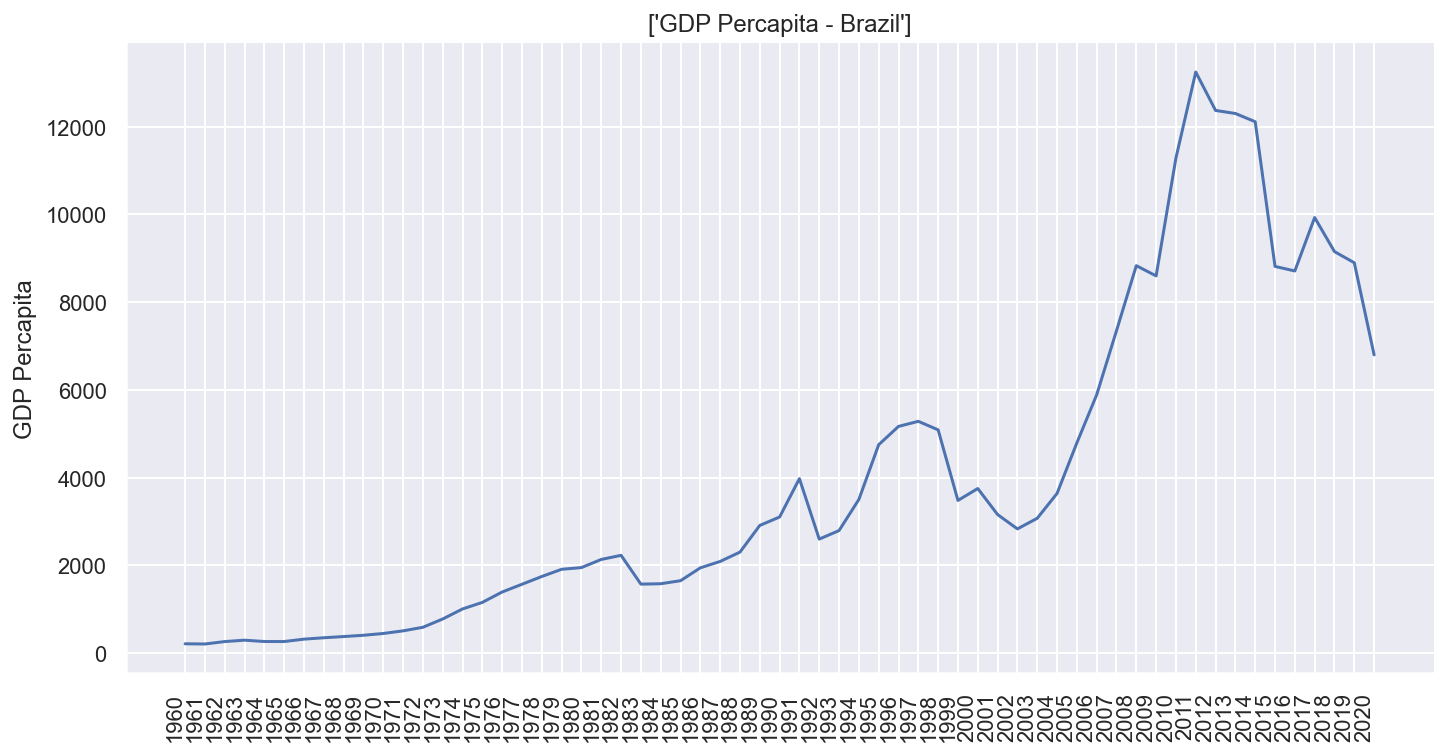
\includegraphics[width=\linewidth]{gdp_graph.PNG}
    \caption{Exemplo de gráfico gerado com os dados da API}
\end{figure}

\section{Conclusões}

Este projeto teve como objetivo demonstrar a criação, deploy e uso de uma API.
Ainda há melhorias para fazer como por exemplo possibilitar o filtro por região, nível de renda do país e faixa de ano dos dados. 
Foi ótimo poder fazer esse projeto pois nunca tinha criado uma API, e muito menos feito o deploy, então sem dúvidas aprendi demais durante todo o processo.



\end{document}
